\chapter{Antecedentes}
\label{ch:CH01}
\ihead[]{Cap\'itulo 1: Antecedentes}
%%%%%%%%%%%%%%%%%%%%%%%%%%%%%%%%%%%%%%%%%%

En este capítulo, se presentan los antecedentes para contextualizar la problemática del presente trabajo de investigación. A su vez, se detallan los objetivos y el alcance de la propuesta de solución que serán desarrollados en capítulos posteriores siguiendo una metodología de diseño mecatrónico.
\section{Problemática y Motivación}
    \label{sec:CH01_Problematica}
    Los motores de corriente continua \ac{DC} son componentes que están presentes en una amplia gama de dispositivos y sistemas. Por ejemplo, estos se encuentran en electrodomésticos de uso diario, como secadores de cabello, cepillos de dientes eléctricos y juguetes electrónicos. Sin embargo, estos componentes desempeñan un papel fundamental en el sector industrial, donde se destacan por su capacidad de proporcionar un control preciso de torque y velocidad. 
     
    La relevancia de los motores \ac{DC} en la industria se refleja en el comportamiento del mercado global, que ha experimentado un crecimiento sostenido en los últimos años y proyecta un incremento continuo hasta 2030. Según \textcite{estadistica_motorDC}, se estima que la tasa de crecimiento anual del mercado de motores \ac{DC} alcanzará un 5.3\% en los próximos años, como se muestra en el gráfico de la Figura \ref{fig:estadistica_problemática}. Este crecimiento está impulsado por su demanda en  aplicaciones, tanto en el ámbito industrial como en el sector automotriz, donde estos motores son fundamentales para garantizar el funcionamiento de las máquinas utilizadas en la industrias. La tendencia mostrada subraya la necesidad de asegurar que los motores \ac{DC} conserven altos estándares de calidad, especialmente en mercados donde la producción en masa es clave para satisfacer la demanda. 
    % \begin{figure}[t]
    % \centering
    % 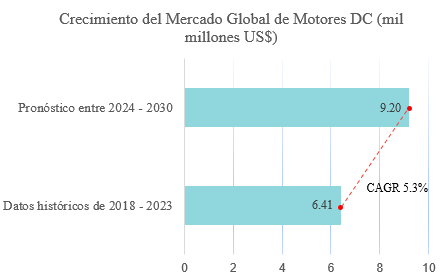
\includegraphics[width=0.6\textwidth]{CHPTRS/CH01_INT/Fig/01_EstudioMercado.png}
    % \caption{Estudio de mercado sobre motores \ac{DC} obtenido de un estudio de la consultora Maximize Market Research \textcite{estadistica_motorDC}}
    % \label{fig:estadistica_problemática}
    % \end{figure}

    
    \begin{figure}[!ht]
    \centering
    \begin{tabularx}{\linewidth}{>{\centering\arraybackslash}X}
        % Fila 1: imagen
        \begin{subfigure}[t]{0.6\linewidth}
            \centering
            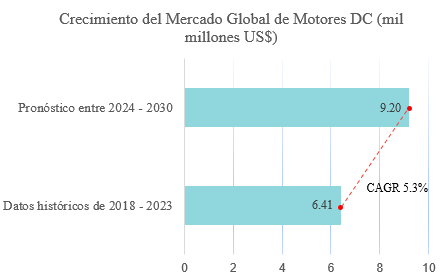
\includegraphics[width=\linewidth]{CHPTRS/CH01_INT/Fig/01_EstudioMercado.png}
        \end{subfigure}
        \\[2mm]
        % Fila 2: nota
        \begin{subfigure}[t]{\linewidth}
            \caption*{\textit{Nota: Figura elaborada a partir de datos de \textcite{estadistica_motorDC}.}}
        \end{subfigure}
    \end{tabularx}
    \caption{Estudio de mercado sobre motores \ac{DC} .}
    \label{fig:estadistica_problemática}
\end{figure}

        
    En el campo de la ingeniería mecatrónica, los motores \ac{DC} son ampliamente utilizados debido a su capacidad para proporcionar un control preciso de velocidad y torque, características esenciales en proyectos de robótica y automatización de procesos \parencites{est_matlab_art_mexicano}. Dos proyectos mecatrónicos relevantes donde se utilicen estos componentes, se presentan a continuación. Ambos proyectos son investigaciones desarrolladas por la empresa \textcite{maxon_group}, reconocida por su especialización en el diseño, desarrollo y fabricación de motores eléctricos de alta calidad.  
    
    El primero de estos proyectos es un robot humanoide llamado Romeo, accionado exclusivamente por motores \ac{DC} de esta empresa. Este robot, ilustrado en la Figura \ref{fig:romeo}, está diseñado para asistir a personas de edad avanzada. Romeo está equipado con 37 motores de alta precisión que controlan sus articulaciones, permitiéndole desplazarse, interactuar y colaborar en las tareas del hogar que, debido a problemas de salud u otras limitaciones, los adultos mayores no puedan realizar.
    
    El segundo proyecto está relacionado con el rover \textit{Perseverance}, diseñado para la exploración y navegación en Marte. En colaboración con la NASA, la empresa \textcite{maxon_group} fue responsable de probar el sistema del rover \textit{Perseverance}, el cual cuenta con diez motores eléctricos que realizan funciones críticas. Entre las funcionalidades que realiza este rover se encuentra el accionar el brazo robótico encargado de transferir muestras entre estaciones, además de sellar y posicionar los contenedores de estas muestras. El rover \textit{Perseverance} se presenta en la Figura \ref{fig:perseverance}.    
%%%%%%%%%%%%%%%%%%%%%%%%%%%%%%%%%%%%%%%%%%%%%%%%%%%%%%%%%%%%%%%%%%%%%%%%%%%%%%%%%%
% NOTA: Para usar una figura al lado de otra se puede usar el paquete \tabularx, la idea es:
%       COL-1     COL-2
%   |----------*-----------*
%   | fig.A    | fig.B     |  FILA-1
%   |----------*-----------*
%   |caption a | caption b |  FILA-2
%   |label a   | label b   |
%   |----------*-----------*
%   |Nota a    | Nota b    |  FILA-3
%   |----------*-----------*
%   caption figura en general
%   label Figura en general.
\begin{figure}[!ht]
    \begin{tabularx}{\linewidth}{*{2}{>{\centering\arraybackslash}X}}
        % FILA-1, COL-1.
        \begin{subfigure}[t]{0.45\textwidth}
            \centering
            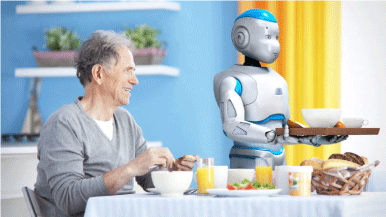
\includegraphics[width=.9\linewidth]{CHPTRS/CH01_INT/Fig/02a_Maxon-Romeo.png}
            %\label{fig:romeo} %LABEL ESTA DESPUES
        \end{subfigure}
        & %Nueva Columna, es decir: % FILA-1, COL-2
        \begin{subfigure}[t]{0.45\textwidth}
            \centering
            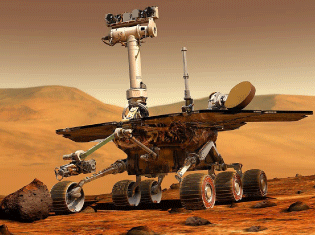
\includegraphics[width=.68\linewidth]{CHPTRS/CH01_INT/Fig/02b_Perseverance.png}
        \end{subfigure}
        \\ %Nueva Fila, es decir: % FILA-2, COL-1
        \begin{subfigure}[t]{0.8\linewidth}
            \caption{Imagen referencial del robot humanoide Romeo}
            \label{fig:romeo}
        \end{subfigure} 
        & %Nueva Columna, es decir: % FILA-2, COL-2
        \begin{subfigure}[t]{0.8\linewidth}
            \caption{Imagen referencial del rover \textit{Perseverance}}
            \label{fig:perseverance}
        \end{subfigure}
        \\ %Nueva Fila, es decir: % FILA-3, COL-1
        \begin{subfigure}[t]{\linewidth}
            \caption*{\textit{Nota: Figura tomada de la página oficial de \linebreak\textcite{maxon_group}}}
        \end{subfigure} 
        & %Nueva Columna, es decir: % FILA-3, COL-2
        \begin{subfigure}[t]{\linewidth}
            \caption*{\textit{Nota: Figura tomada de la página oficial de \linebreak\textcite{maxon_group}}}
        \end{subfigure}
    \end{tabularx}
    \caption{Ejemplos de aplicaciones reales que utilizan motores \ac{DC}}
    \label{fig:figuraEnGeneral}
\end{figure}
%%%%%%%%%%%%%%%%%%%%%%%%%%%%%%%%%%%%%%%%%%%%%%%%%%%%%%%%%%%%%%%%%%%%%%%%%%%%%%%%%
    Para ambos proyectos es fundamental el uso de motores que cumplan con los más altos estándares de calidad, los cuales son previamente sometidos a pruebas en laboratorios altamente especializados. Sin embargo, en el contexto peruano no se dispone de servicios de caracterización de motores eléctricos. Según el profesor Joaquín Gonzales, docente de Máquinas Eléctricas de la \ac{PUCP} e integrante del Centro de Investigación Arvico, “en el Perú, simplemente se opta por comprar \ac{HW} que permita el control de motores DC” (J. Gonzales, comunicación personal, 2024). 
    
    Por todo lo expuesto es conveniente conocer con exactitud los parámetros eléctricos y mecánicos de un motor \ac{DC}, debido a que estos determinan la respuesta del motor y, en consecuencia, influyen en la eficiencia y precisión de este. Además, existen \ac{SW} como \textcite{etap} o MATLAB que permiten realizar estas estimaciones de manera precisa. Sin embargo, todo esto implica un alto costo económico y, aunque son opciones eficaces, no siempre son viables para proyectos de menor escala o presupuestos limitados, lo que resalta la necesidad de alternativas más accesibles.
     
   La principal motivación de este trabajo de investigación es proporcionar a estudiantes de ingeniería mecatrónica y carreras afines una máquina capaz de caracterizar motores DC, facilitando su uso en proyectos y prácticas académicas. Esto fomenta el desarrollo de técnicas de control más precisas con estos componentes durante una etapa de aprendizaje, lo cual puede resultar valioso al integrarse a la industria. Asimismo, en el ámbito industrial, se espera que esta solución sea útil para empresas en el Perú que requieran asesoramiento o herramientas de control de calidad para los motores empleados en aplicaciones de automatización y control, considerando que, como se mencionó, en el país no existe el \textit{know-how} necesario para la caracterización de motores.

    % \section{Propuesta de solución}
    % \label{sec:CH01_Propuesta}
    % Este trabajo se enfocará en el diseño e implementación de un sistema mecatrónico para la estimación de parámetros de motores \ac{DC}. El sistema estará compuesto por dos partes, una de \ac{HW} y otra de \ac{SW}. La primera se encargará del acondicionamiento de señales y la recolección de datos, que luego serán procesados por el algoritmo de estimación de parámetros. La segunda consistirá en el desarrollo del \ac{SW}, el cual se llevará a cabo, inicialmente, en la plataforma MATLAB. Se implementará un algoritmo capaz de estimar los parámetros de los motores \ac{DC}, para ello se desarrollará una interfaz gráfica de usuario \ac{GUI} que permita procesar, visualizar y verificar la precisión del algoritmo. La solución será semi-automatizada, ya que existen motores con diferentes rangos de voltaje y dimensiones. Por lo tanto, se espera que el usuario ajuste manualmente el sistema para adaptarlo al motor que será analizado y en este caso la solución será validada con motores de hasta 12 voltios.
    
    \section{Objetivos}
\label{sec:CH01_Objetivos}
El presente trabajo de investigación tiene como objetivo principal, implementar y validar un diseño de un banco de pruebas para la estimación de  parámetros de motores \ac{DC}. Para lograr este propósito se han definido cinco objetivos específicos, los cuales permitirán estructurar y guiar el desarrollo de la solución óptima.

\subsection{Objetivo general}
El objetivo general es diseñar e implementar un sistema mecatrónico para la estimación de parámetros de motores \ac{DC} utilizando la metodología VDI 2221 y VDI 2206 \autocite{vdi2206} \autocite{vdi2221} y se espera tener, según los niveles de \ac{TRL}, una solución con un nivel de madurez tecnológica TRL4 \autocite{trl}, luego de las respectivas validaciones.

\subsection{Objetivos específicos}
\begin{itemize}
    \item Diseñar el subsistema mecánico del banco: piezas y acoples para el censado de velocidad angular con el encoder elegido, adaptables a las distintas geometrías y ejes de motores en el rango de $12$\,V; soportes de prueba para el motor; un chasis que sirva para conectar correctamente la alimentación de la máquina, del motor y los cables que tendrán los datos del proceso de censado; y una carcasa que indique al usuario si el banco está encendido y soporte todos los componentes de la solución final. Para ello, se utilizarán estándares para los soportes de motores DC, se seleccionarán los conectores y luces de indicación para tener en cuenta las dimensiones de estos componentes, se procederá a medir correctamente y, apoyados con un \ac{SW} de diseño \ac{CAD}, se brindará la correcta posición de todos los componentes, diseñando en el \ac{SW} \ac{CAD} un acople de acuerdo a las necesidades de geometría de los motores que se utilizarán. Para que, todo esto se utilice con la finalidad de apoyar a los demás subsistemas como el electrónico, que necesitará que algunos componentes estén fijos durante las pruebas como el encoder para censar la velocidad, o los conectores de potencia y de información que se conectarán a la computadora donde se realizará la estimación.

    \item Seleccionar los componentes necesarios para el correcto control y comunicación entre el \ac{HW} físico y el \ac{SW} con el algoritmo de estimación, por medio de una \ac{PCB} de control y otra \ac{PCB} dedicada al acondicionamiento y censado de las principales variables del motor. Para ello, se investigarán circuitos que permitan la conexión entre reguladores de voltaje, interfaces y módulos de comunicación, sensores de velocidad, \textit{drivers} para probar el motor y un microcontrolador capaz de controlar toda la experiencia de toma de datos con la información proporcionada por la \ac{GUI}. Todo ello deberá será de suma importancia debido a que el dominio electrónico se encargará de brindar los datos que servirán para la estimación de los parámetros del motor que se quiera caracterizar.

    \item Desarrollar el \ac{SW} que implemente un algoritmo de identificación de parámetros en línea mediante una \ac{GUI} y controle el \ac{HW} del banco de pruebas vía Ethernet. Para ello, se programará la \ac{GUI} para configurar ensayos, enviar comandos al microcontrolador, automatizar la adquisición, visualizar resultados y registrar datos. Para que la identificación se ejecute en línea de forma confiable, se asegurará la comunicación entre \ac{HW} y \ac{SW} eligiendo correctamente el \ac{HW} necesario para ello en los dominios previamente mencionados.

    \item Validar la solución propuesta mediante indicadores cuantitativos de desempeño en al menos dos motores con sus respectivas fichas técnicas en el rango de $12$\,V. A su vez se busca comparar la estimación brindada por el algoritmo a implementar con métodos existentes de estimación de parámetros de motores \ac{DC} descritos en la literatura, considerando costos de implementación y exactitud. 
\end{itemize}
            
    \section{Alcance}
    \label{sec:Alcance}
    Se busca que la solución final alcance un nivel de madurez tecnológica TRL4 \autocite{trl}. Asimismo, se estimará el costo de fabricación del prototipo con el fin de evaluar su viabilidad técnica y económica. Los resultados se validarán mediante métodos de identificación de parámetros descritos en el capítulo \ref{ch:CH02}. Toda investigación y las aproximaciones propuestas se basan en el modelo lineal de los motores de corriente continua presentado en dicho capítulo. Se busca implementar todo el \ac{HW} en su totalidad del concepto ganador y su integración con el \ac{SW} del diseño; de no ser posible culminar esta integración, se dividirá en dos etapas: sensado de datos con el \ac{HW} diseñado y  estimación de parámetros en forma \textit{offline}. Durante el diseño de la solución óptima se optó por indicar que el usuario deberá brindar una fuente externa de acuerdo al voltaje nominal del motor a ensayar. Esta decisión se justifica en el capítulo \ref{ch:CH03}, dedicado al diseño conceptual del prototipo.
    % Cambiar el título de la tesis, al final se compararán los resultados entre motores con y sin caja reductora para ver si varía (eso puede ir en pruebas en alguno de los capítulos de diseño o en Anexos)
    
    \section{Metodología}  
    En el desarrollo de este trabajo de investigación se usará la metodología VDI 2221 y VDI 2206, ambas desarrolladas por la ``Sociedad de Ingenieros Alemanes'' \autocite{vdi2206}. 
    Según lo descrito anteriormente, se organizará el documento de la siguiente manera:
    \begin{itemize}
        \item En el capítulo \ref{ch:CH02} se presentará al lector los conceptos teóricos detrás de la estimación de parámetros de motores \ac{DC}. Seguidamente se presentará el modelo matemático de un motor \ac{DC} y los parámetros que conforman la dinámica del mismo, a su vez de detallarán los algoritmos más usados para la caracterización de motores \ac{DC}, según \autocite{Electronics}.
        
        \item En el capítulo \ref{ch:CH03} se abordará el diseño conceptual del sistema a desarrollar, presentando una lista de requerimientos que delimitará el funcionamiento que deberá cumplir la solución diseñada en los capítulos posteriores. Esta lista expresa principalmente requerimientos cuantitativos, lo que permitirá realizar un seguimiento para verificar que se cumplan los valores correspondientes. Para su elaboración, se investigaron antecedentes de trabajos afines y se entrevistó al actual director de la Maestría en Control y Automatización de la \ac{PUCP}, quien arguye con su perspectiva y experiencia para acotar los requerimientos del sistema presentados en esta tesis.
        
        \item En el capítulo 3 se presentarán empresas de renombre que ofrecen motores DC junto con sus respectivas especificaciones, así como software destinado a la estimación de parámetros. Además, se analizarán artículos y papers de aplicaciones previas que expongan resultados de soluciones utilizadas para estimar parámetros de motores DC. Asimismo, se incluirá una lista de los componentes necesarios para la estimación de parámetros, como sensores de corriente, encoders para medir la velocidad angular del motor, entre otros componentes.
        
        \item A su vez, en el capítulo \ref{ch:CH03} se identificarán las señales de entrada del sistema y se definirán las salidas que contará el sistema base de la cual partirá la estructura de funciones del sistema. Luego de ello se presentarán los componentes/medios necesarios para las pruebas con los motores y la adquisición data relevante para el procesamiento del algoritmo de estimación. Se propondrán al menos tres soluciones, conforme a la norma, y que serán evaluadas mediante un análisis técnico-económico, en base a ello se elegirá un sólo concepto de solución que se tomará como base para el diseño del estimador de parámetros. 
        
        \item Posteriormente, se procederá a diseñar cada una de las funciones de los dominios mecánicos, electrónicos, software y de control que contará la solución óptima elegida para, finalmente, ser implementada y testeada con diferentes tipos de motores para comprobar la estimación de parámetros.
        
        \item Finalmente, se presentarán los resultados obtenidos por el concepto de solución diseñado. En caso no se llegase a cumplir con todos los objetivos propuestos o los requerimientos brindados, se optará por dar recomendaciones o alternativas que aseguren la correcta estimación de parámetros de motores \ac{DC}.
    \end{itemize}
    
    
    